\section{Deadlock}
Si è in deadlock quando un gruppo di processi è in attesa di acquisire una risorsa posseduta da un altro processo nello stesso gruppo.

Per esempio supponiamo di avere due risorse singole A e B e di avere i seguenti processi:
\begin{verbatim}
    P1:
        wait(A)
        wait(B)
    
    P2:
        wait(B)
        wait(A)
\end{verbatim}
Se il processo $P_1$ riesce ad acquisire A ed il processo $P_2$ ad acquisire B ognuno dei due blocca l'altro dall' accesso ad entrambe le risorse: siamo in deadlock!

\subsection{Grafo di allocazione delle risorse}
E' un grafo i cui nodi sono partizionati in due categorie:
\begin{itemize}
    \item $P$: l' insieme dei processi
        \begin{figure}[H]
            \centering
            
\includegraphics[width=25px]{images/8_Deadlock/process.png}
        \end{figure}
    \item $R$: l' insieme delle risorse:
        \begin{itemize}
            \item A singola istanza: ne ho solo una e la assegno ad un processo per volta
                \begin{figure}[H]
                    \centering
                    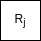
\includegraphics[width=25px]{images/8_Deadlock/single_resource.png}
                \end{figure}
            \item A multipla istanza: ne ho $n$ e posso assegnarla ad $n$ processi diversi alla volta
                \begin{figure}[H]
                    \centering
                    
\includegraphics[width=25px]{images/8_Deadlock/multiple_resource.png}
                \end{figure}
        \end{itemize}
\end{itemize}
Mentre gli archi possono essere di due tipi:
\begin{itemize}
    \item Arco di richiesta: se va da un processo ad una risorsa
        \begin{figure}[H]
            \centering
            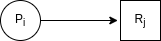
\includegraphics[width=100px]{images/8_Deadlock/request_edge.png}
        \end{figure}
    \item Arco di assegnamento: se va da una risorsa ad un processo
        \begin{figure}[H]
            \centering
            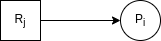
\includegraphics[width=100px]{images/8_Deadlock/assignment_edge.png}
        \end{figure}
\end{itemize}

\subsubsection{Grafo possesso-attesa}
Concordiamo che l'accesso alla risorsa va fatto seguendo il protocollo:
\begin{itemize}
    \item Prologo: controllo se la risorsa è disponibile ed eventualmente la acquisisco, altrimenti rimango in attesa che si liberi
    \item Utilizzo: ho la risorsa e la posso utilizzare
    \item Epilogo: rilascio la risorsa a qualcun altro
\end{itemize}

Se disegnamo anche le attese sulle risorse occupate possiamo ottenere il grafo \emph{possesso-attesa}.

\subsection{Caratterizzazione del deadlock}
Si può andare in deadlock se si verificano simultaneamente queste 4 condizioni:
\begin{itemize}
    \item Mutua esclusione: se non ho sezioni critiche non posso avere deadlock
    \item Hold \& wait: un job che ha una risorsa si mette in attesa di un' altra
    \item No preemption: la risorsa può essere rilasciata solo volontariamente dal job, non posso revocargliela
    \item Attesa ciclica: esiste un insieme di processi $\{ P_0, P_1, \_, P_n \}$ in cui $P_0$ è in attesa di una risorsa che ha $P_1$, $P_1$ è in attesa di una risorsa che ha $P_2$, ..., $P_n$ è in attesa di una risorsa che ha $P_0$.
    Si tratta di un ciclo nel grafo di allocazione delle risorse
\end{itemize}

NB: le quattro condizioni assieme sono \emph{condizione necessaria}!

NB: avere un ciclo nel grafo di allocazione delle risorse è una \emph{condizione necessaria} affinché ci sia un deadlock, tuttavia se le risorse sono tutte a singola istanza diventa una \emph{condizione sufficiente}.
\begin{figure}[H]
    \centering
    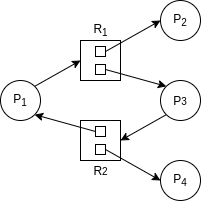
\includegraphics[width=140px]{images/8_Deadlock/loop_no_deadlock.png}
\end{figure}
Abbiamo un ciclo ma non abbiamo un deadlock perché $P_2$ e $P_4$ possono terminare in qualsiasi momento e restituire le risorse in modo che le richieste di $P_1$ e $P_3$ vengano soddisfatte.
\begin{figure}[H]
    \centering
    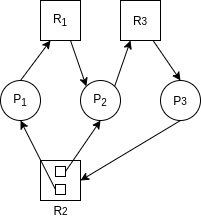
\includegraphics[width=125px]{images/8_Deadlock/loop_deadlock.png}
\end{figure}
In questo secondo caso oltre al ciclo abbiamo anche un deadlock.

\subsection{Gestione del deadlock}
Possiamo gestire il deadlock in 3 modi:
\begin{itemize}
    \item Assicurarsi che il sistema non entri mai in deadlock:
    \begin{itemize}
        \item \emph{deadlock prevention} - prevenzione statica
        \item \emph{deadlock avoidance} - prevenzione dinamica
    \end{itemize}
    \item Accorgersi del deadlock e riparare la situazione: \emph{deadlock detection e recovery}
    \item Ignorare completamente il problema (approccio usato da UNIX e molti altri sistemi operativi)
\end{itemize}

\subsubsection{Deadlock prevention}
Possiamo provare ad eliminare le sorgenti di deadlock quando possibile semplicemente tramite una analisi statica del comportamento del programma, cioè senza eseguirlo:

Posso limitare la mutua esclusione alle sole risorse condivise.

Per risolvere la questione della hold \& wait potrei pensare di:
\begin{itemize}
    \item obbligare il programma a chiedere tutte le risorse all' inizio bloccando eventuali richieste eseguite in secondi momenti
    \item permettere ad un processo di richiedere risorse solo se non ne ha nessuna
    \item permettere l' accesso ad una sola risorsa per volta
\end{itemize}
Queste soluzioni sono altamente limitanti, possono portare alla starvation ed a volte sono addirittura impraticabili in quanto non sempre è possibile conoscere le risorse di cui un processo avrà bisogno a tempo di esecuzione.
Prevede inoltre un grande sforzo da parte del programmatore in quanto deve ripensare al codice in modo che soddisfi queste richieste.

Se un processo prova a richiedere una risorsa che al momento è occupata allora rilascia tutte le risorse che ha e si mette in attesa di tutte le risorse che aveva più quella che ha richiesto; il processo verrà riavviato una volta che tutte le risorsa saranno disponibili allo stesso momento.
Questo meccanismo aggiunge un forte overhead in quanto bisogna salvare lo stato delle risorse: per alcune è semplice (ad esempio posso liberare la memoria tramite la paginazione su domanda) per altre è difficile se non impossibile, come nel caso di alcune periferiche.

Per risolvere l' attesa ciclica posso imporre un ordinamento alle risorse e quindi obbligare i programmi a richiedere le risorse seguendo questo ordine, impedendo qualsiasi richiesta out of order.

In definitiva sono tecniche che si posso usare in taluni casi ma non garantiscono la prevenzione al 100\% e non sempre sono utilizzabili.

\subsubsection{Deadlock avoidance}
Per queste pratiche è necessario che un processo dichiari, prima della esecuzione, di quali e quante risorse avrà bisogno al massimo.
Il sistema poi si occuperà di monitorare in continuazione lo stato dei processi e delle risorse per assicurarsi che non possa mai esserci una attesa circolare.
Alla richiesta di allocazione di una risorsa quindi controllo cosa potrebbe succedere se la concedessi, se mi porta in uno stato insicuro non rendo disponibile la risorsa e metto il processo in pausa.
Questo metodo può portare il processo in uno stato di hold \& wait ma è conscio e controllato.

Definiamo prima di tutto cosa è un \emph{safe state}: un sistema è in safe state se esiste un ordinamento $<P_1, P_2, \_, P_n>$ di tutti i processi del sistema tale che tutte le richieste che il processo $P_i$ può ancora eseguire saranno soddisfatte tramite le risorse correntemente libere $+$ quelle acquisite dai processi $P_j$ con $j < i$.
Cioè se $P_i$ farà delle richieste deve poterle avere soddisfatte dalle risorse che ci sono già adesso oppure aspettando la fine dei processi prima di lui nella sequenza e prendendo le loro risorse.

Si dimostra infatti che se si rimane in un safe state non ci possono essere deadlock, invece se si va in un unsafe state la probabilità di deadlock c'è.
Possiamo quindi costruire algoritmi che controllino di permanere in un safe state ad ogni richiesta.
\\
\\
Se ho solo risorse a singola istanza posso tenere in memoria il grafo di allocazione delle risorse così formato:
\begin{itemize}
    \item \emph{claim edge}: ramo che indica che $P_i$ potrebbe richiede la risorsa $R_j$, l'arco è tratteggiato e va dal processo alla risorsa
    \item \emph{request edge}: quando il processo $P_i$ richiede la risorsa $R_j$, è una fase transitoria che fa partire l' algoritmo
    \item \emph{assignment edge}: quando la risorsa $R_j$ è assegnata al processo $P_i$, l'arco è continuo e va dalla risorsa al processo
    \item \emph{wait edge}: quando il processo ha richiesto una risorsa ma è bloccata e quindi si mette in attesa, l' arco è continuo e va dal processo alla risorsa 
\end{itemize}
e controllare ad ogni richiesta che il grafo ottenuto allocando la risorsa al processo che la chiede non contenga un ciclo.

Supponiamo di avere il seguente grafo di allocazione delle risorse:
\begin{figure}[H]
    \centering
    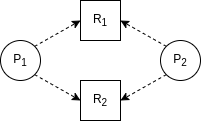
\includegraphics[width=125px]{images/8_Deadlock/first_state.png}
\end{figure}
Supponiamo poi che $P_1$ chieda $R_1$ e che gli venga concessa, poi che $P_2$ chieda $R_2$, a questo punto il nostro algoritmo scatta e valuta il seguente grafo:
\begin{figure}[H]
    \centering
    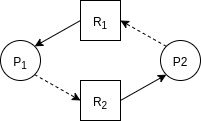
\includegraphics[width=125px]{images/8_Deadlock/second_state.png}
\end{figure}
Il grafo che si otterrebbe se la risorsa venisse concessa produce un ciclo quindi finiamo in un unsafe-state, non possiamo concedere la risorsa.

Supponiamo invece che $P_1$ chieda $R_1$ e gli venga concessa, che $P_2$ chieda $R_2$ e gli venga concessa e successivamente $P_2$ chieda $R_1$, a questo punto l' algoritmo produce il seguente grafo:
\begin{figure}[H]
    \centering
    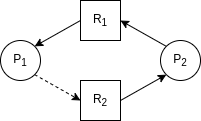
\includegraphics[width=125px]{images/8_Deadlock/third_state.png}
\end{figure}
Anche in questo caso si è venuto a creare un ciclo, dunque allocando la risorsa si andrebbe in uno stato unsafe!
\\
\\
Se ho risorse a multipla istanza devo ricorrere all' \emph{algoritmo del banchiere}: supponiamo di avere $n$ processi e $m$ tipi di risorse, costruiamo le seguenti strutture:
\begin{itemize}
    \item vettore di lunghezza $m$ \emph{available}: mantiene il numero di istanze di ogni risorsa che sono disponibili
    \item matrice $n \times m$ \emph{max}: mantiene il numero di risorse per ogni tipo che ogni processo può richiedere al massimo
    \item matrice $n \times m$ \emph{allocation}: mantiene il numero di risorse per ogni tipo allocate ad ogni processo
    \item matrice $n \times m$ \emph{need}: mantiene il numero di risorse per ogni tipo che mancano ad ogni processo per terminare. Si può ottenere come:
    $$ need[i][j] = max[i][j] - allocation[i][j] $$
\end{itemize}
Ad ogni richiesta di una risorsa si fa partire l' algoritmo:
\begin{enumerate}
    \item si creano i vettori \emph{work} e \emph{finish} di lunghezza $m$ ed $n$ e li si inizializzano:
    $$ work = available $$
    $$ finish[i] = false $$

    \item trovare una $i$ tale che:
    $$ finish[i] = false$$
    $$ need_i \leq work $$
    cioè trovare un processo che non abbia già flaggato come finito e che riuscirebbe a finire con le risorse disponibili in quel momento.
    Se non ci sono processi tali andare allo step 4.

    \item aggiornare le strutture:
    $$ work = work + allocation_i $$
    $$ finish[i] = true $$
    cioè segnala il processo trovato come finito ed aggiungi le risorse che aveva allocato a quelle disponibili.
    Tornare allo step 2.
    
    \item Se \emph{finish} è popolato solo da \emph{true} allora il sistema è in un safe state
\end{enumerate}

In definitiva quando un processo chiede alcune risorse:
\begin{enumerate}
    \item Si controlla che la richiesta non faccia eccedere il numero massimo di risorse che il processo può acquisire
    \item Se la risorsa non è disponibile metto in attesa il processo
    \item Se la risorsa è disponibile o torna disponibile aggiorno le strutture dati:
    $$ Available = Available - Request_i $$
    $$ Allocation_i = Allocation_i + Request_i $$
    $$ Need_i = Need_i - Request_i $$
    si esegue l' algoritmo, se è in safe state allora si allocano effettivamente le risorse, se non è safe si fa aspettare il processo e si ripristinano le strutture a com'erano prima dell' aggiornamento
\end{enumerate}

\subsubsection{Deadlock detection}
Questa tecnica prevede che il sistema entri in deadlock, un algoritmo parta periodicamente ed eventualmente lo rilevi, una volta rilevato si applicano degli schemi di recupero.

Per risorse a singola istanza possiamo mantenere in memoria un grafo \emph{wait-for} in cui i nodi sono i processi e gli archi indicano che un processo è in attesa di un altro. Questo grafo può essere ottenuto a partire dal grafo di allocazione delle risorse:
\begin{figure}[H]
    \centering
    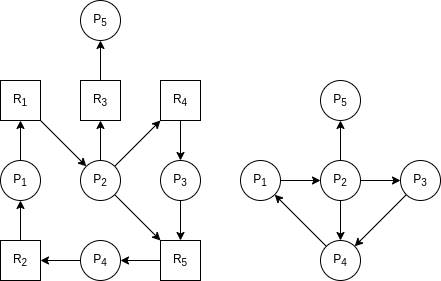
\includegraphics[width=275px]{images/8_Deadlock/wait_for_graph.png}
\end{figure}
Se si trova un ciclo all' interno del grafo allora c' è un deadlock e si provvede a risolverlo.
\\
\\
Per risorse multiple invece si deve mantenere in memoria:
\begin{itemize}
    \item \emph{available}: vettore di lunghezza $m$ che indica per ogni tipo di risorsa quante ce ne sono disponibili
    \item \emph{allocation}: matrice $n \times m$ che indica per ogni processo quante risorse di ogni tipo possiede
    \item \emph{request}: matrice $n \times m$ che indica le risorse che stanno richiedendo in questo momento i processi
\end{itemize}
Successivamente si procede con il seguente algoritmo:
\begin{enumerate}
    \item si costruiscono gli array \emph{work} e \emph{finish} di lunghezze $m$ ed $n$:
    $$ work = available $$
    \begin{equation}
        finish[i] = 
        \begin{cases}
            false \text{ se $allocation_i$} \neq 0 \\
            true \text{ se $allocation_i$} = 0 \\
        \end{cases}
    \end{equation}
    
    \item si trova un indice $i$ tale che:
    $$ finish[i] = false $$
    $$ request_i \leq work $$
    se non ne trovo alcuno andare al passo 4
    
    \item aggiornare:
    $$ work = work + allocation_i $$
    $$ finish[i] = true $$
    andare allo step 2
    
    \item se $finish$ contiene alcuni valori falsi allora il sistema è in deadlock, in particolare se $finish[i] = false$ allora $P_i$ è in deadlock 
\end{enumerate}
Questo algoritmo può essere eseguito in $O(m \cdot n^2)$.
\\
\\
Una volta definiti gli algoritmi da utilizzare dobbiamo pensare alla temporizzazione della detection.
Si può pensare di lanciare l' algoritmo ogni volta che la richiesta di un processo porta ad una pausa in quanto potrebbe essere l' inizio di un deadlock.
Questo approccio tuttavia è molto dispendioso in termini di risorse in quanto l' algoritmo di ricerca del ciclo è $O(n^2)$ mentre quello per risorse multiple è $O(m \cdot n^2)$ quindi si ha complessità non indifferente ogni volta che si deve andare in pausa.

Un approccio migliore sarebbe già quello di lanciarlo periodicamente per controllare lo stato generale dei processi.
Possiamo studiare la frequenza con la quale un deadlock si verifica nel sistema in analisi e tarare il periodo su questo tempo.
Se il deadlock è imprevedibile possiamo unire la temporizzazione all' utilizzo della CPU, se essa cala molto o è sotto un certo livello possiamo lanciare l' algoritmo ed indagare le cause.
\\
\\
In fine dobbiamo decidere che politiche intraprendere quando si rileva un deadlock: principalmente abbiamo l' aborto di uno o più processi o la preemption di qualche risorsa.

Se decidiamo di killare i processi dobbiamo scegliere se killare tutti i processi in deadlock o solo uno e poi rieseguire la detection.
Alcuni criteri con i quali scegliere i singoli processi o l' ordine possono essere:
\begin{itemize}
    \item priorità dei processi
    \item quanto un processo ha già computato e quanto ancora gli manca
    \item le risorse che il processo ha usato
    \item le risorse di cui il processo ha necessità per terminare
    \item quanti processi è necessario terminare
    \item se il processo è interattivo o batch
\end{itemize}

Quando killo un processo o rilevo una risorsa devo eseguire un rollback del processo ad uno stato consistente, per fare ciò è necessario che io salvi alcuni stati intermedi: ad esempio su una wait mi salvo il contesto del processo ed alcune porzioni della sua memoria in modo da poterli ripristinare successivamente in caso di deadlock.
Tutto ciò, ovviamente, aggiunge overhead.

Si noti che se uso un algoritmo basato sulla priorità per scegliere quale processo killare o a quale processo rimuovere le risorse potrei far finire qualche processo in starvation.
